\documentclass[journal]{vgtc}                     % final (journal style)
%\documentclass[journal,hideappendix]{vgtc}        % final (journal style) without appendices
%\documentclass[review,journal]{vgtc}              % review (journal style)
%\documentclass[review,journal,hideappendix]{vgtc} % review (journal style)
%\documentclass[widereview]{vgtc}                  % wide-spaced review
%\documentclass[preprint,journal]{vgtc}            % preprint (journal style)


%% Uncomment one of the lines above depending on where your paper is
%% in the conference process. ``review'' and ``widereview'' are for review
%% submission, ``preprint'' is for pre-publication in an open access repository,
%% and the final version doesn't use a specific qualifier.

%% If you are submitting a paper to a conference for review with a double
%% blind reviewing process, please use one of the ``review'' options and replace the value ``0'' below with your
%% OnlineID. Otherwise, you may safely leave it at ``0''.
\onlineid{0}

%% In preprint mode you may define your own headline. If not, the default IEEE copyright message will appear in preprint mode.
%\preprinttext{To appear in IEEE Transactions on Visualization and Computer Graphics.}

%% In preprint mode, this adds a link to the version of the paper on IEEEXplore
%% Uncomment this line when you produce a preprint version of the article 
%% after the article receives a DOI for the paper from IEEE
%\ieeedoi{xx.xxxx/TVCG.201x.xxxxxxx}

%% declare the category of your paper, only shown in review mode
\vgtccategory{Research}

%% please declare the paper type of your paper to help reviewers, only shown in review mode
%% choices:
%% * algorithm/technique
%% * application/design study
%% * evaluation
%% * system
%% * theory/model
\vgtcpapertype{please specify}

%% Paper title.
\title{Event Hyper Graph}

%% Author ORCID IDs should be specified using \authororcid like below inside
%% of the \author command. ORCID IDs can be registered at https://orcid.org/.
%% Include only the 16-digit dashed ID.
\author{%
  \authororcid{Sam Yu-Te Lee}{},
  \authororcid{Kwan-Liu Ma}{}
}

\authorfooter{
  %% insert punctuation at end of each item
  \item Sam Yu-Te Lee and Kwan-Liu Ma are with University of California, Davis. E-mail: \{ytlee\,$|$\,klma\}@ucdavis.edu\,.
}

%% Abstract section.
\abstract{%
  %
  %% We recommend that you link to your supplemental material here in the abstract, as well
  %% as in the Supplemental Materials section at the end.
  % A free copy of this paper and all supplemental materials are available at \url{https://OSF.IO/2NBSG}.
  TBD
}

%% Keywords that describe your work. Will show as 'Index Terms' in journal
%% please capitalize first letter and insert punctuation after last keyword
\keywords{}

%% A teaser figure can be included as follows
% \teaser{
%   \centering
%   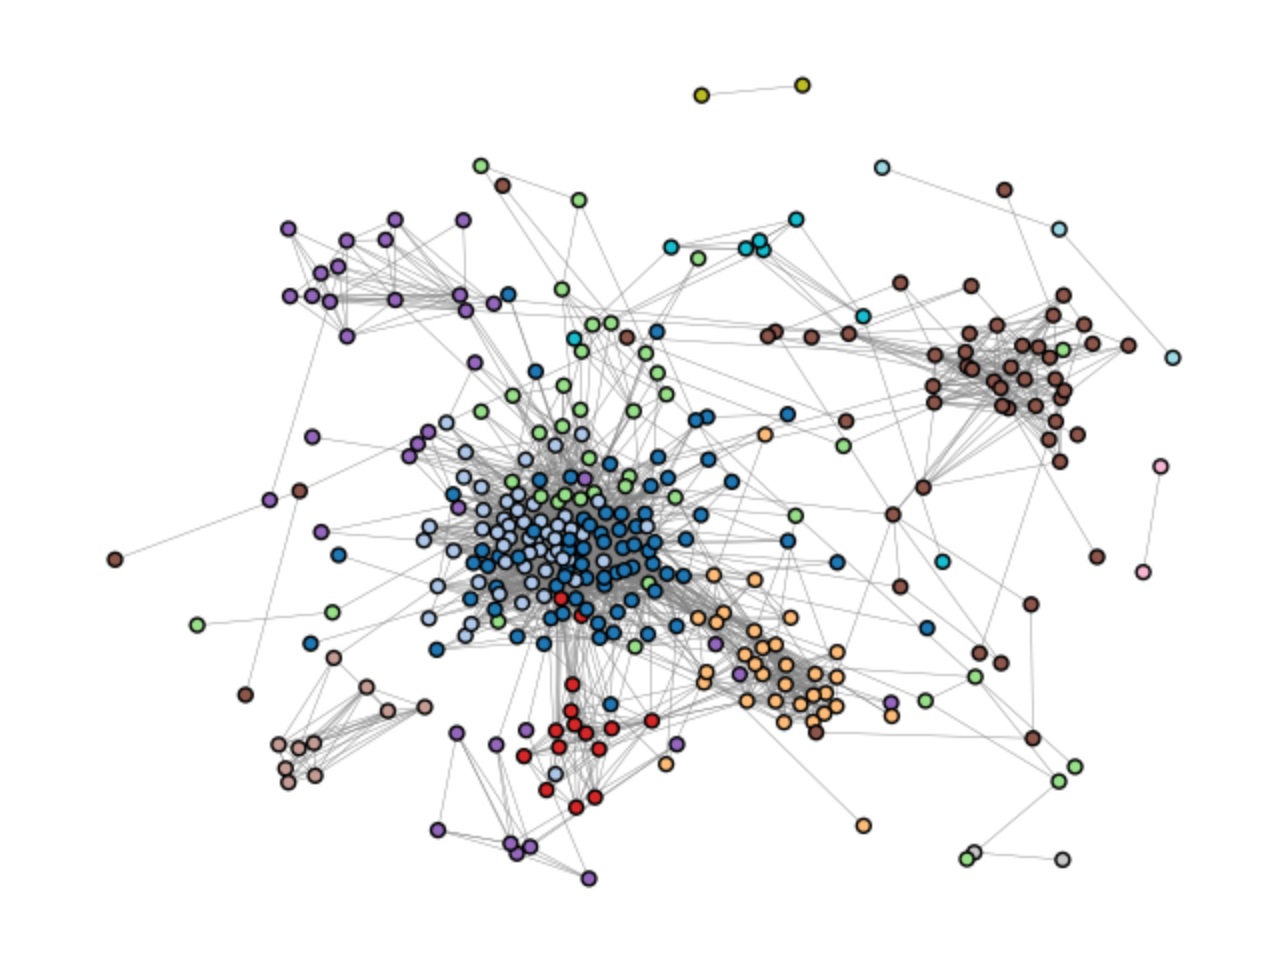
\includegraphics[width=\linewidth]{teaser}
%   \caption{%
%     some caption
%   }
%   \label{fig:teaser}
% }

%% Uncomment below to disable the manuscript note
%\renewcommand{\manuscriptnotetxt}{}

%% Copyright space is enabled by default as required by guidelines.
%% It is disabled by the 'review' option or via the following command:
%\nocopyrightspace


%%%%%%%%%%%%%%%%%%%%%%%%%%%%%%%%%%%%%%%%%%%%%%%%%%%%%%%%%%%%%%%%
%%%%%%%%%%%%%%%%%%%%%% LOAD PACKAGES %%%%%%%%%%%%%%%%%%%%%%%%%%%
%%%%%%%%%%%%%%%%%%%%%%%%%%%%%%%%%%%%%%%%%%%%%%%%%%%%%%%%%%%%%%%%

%% Tell graphicx where to find files for figures when calling \includegraphics.
%% Note that due to the \DeclareGraphicsExtensions{} call it is no longer necessary
%% to provide the the path and extension of a graphics file:
%% 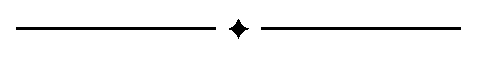
\includegraphics{diamondrule} is completely sufficient.
\graphicspath{{figs/}{figures/}{pictures/}{images/}{./}} % where to search for the images

%% Only used in the template examples. You can remove these lines.
\usepackage{tabu}                      % only used for the table example
\usepackage{booktabs}                  % only used for the table example
\usepackage{lipsum}                    % used to generate placeholder text
\usepackage{mwe}                       % used to generate placeholder figures

\usepackage{color,soul} % added for personal use


%% We encourage the use of mathptmx for consistent usage of times font
%% throughout the proceedings. However, if you encounter conflicts
%% with other math-related packages, you may want to disable it.
\usepackage{mathptmx}                  % use matching math font

\begin{document}

%%%%%%%%%%%%%%%%%%%%%%%%%%%%%%%%%%%%%%%%%%%%%%%%%%%%%%%%%%%%%%%%
%%%%%%%%%%%%%%%%%%%%%% START OF THE PAPER %%%%%%%%%%%%%%%%%%%%%%
%%%%%%%%%%%%%%%%%%%%%%%%%%%%%%%%%%%%%%%%%%%%%%%%%%%%%%%%%%%%%%%%

%% The ``\maketitle'' command must be the first command after the
%% ``\begin{document}'' command. It prepares and prints the title block.
%% the only exception to this rule is the \firstsection command

\maketitle
\section{Introduction}
% summartization -> overview / text mining / transforming large collection of documents into a compact representation / visual summarization
% compact, interactive summary, support analysis, interpretation and trust
% existing methods: based on word co-occurrence -> inaccurate, not able to capture complex relations, not easy to reason why relation exists
% interactions supported: semantic zooming, filtering, highlighting, linking
% analysis supported: global (network statistics, communities) vs. local (paths, motifs)
% 
In text analysis, providing a compact overview of a large collection of documents is a common yet challenging task.
A large collection of documents, or a corpus, could contain multiple interesting characteristics, while the analyst may not already know what to expect.
State-of-the-art techniques can be mainly divided into two categories: word clouds based and topic models based, each having its own advantages and disadvantages.
Word clouds are easy to understand and can be generated quickly, but they are not able to capture the relationships between words and support for further analytical tasks~\cite{viegas2008timelines}.
Topic models can capture the relationships between words, but they are not easy to understand and require parameter tuning~\cite{chuang2013topicdiagnostic}.
The ability to model complex relations lie within the text and interpretability are two important factors to consider when providing a compact overview of a corpus, and they are often in conflict with each other.
Word clouds and topic models lie on the two extremes: word clouds are easy to understand but too simple to capture complex relations, and topic models are able to capture complex relations but not easy to understand.

In addition, a common assumption shared among text analysis methods (not limited to word clouds and topic models) is that each document is a bag of words, and words appearing near to each other indicate meaningful relations.
There are two main problems with this assumption.
First, the fact that meaningful relations between words are informed solely by their co-occurring frequency indicates that the relation is unknown.
Co-occurring frequency merely serves as a signal for the possibility that a relation exists.
Many visual analytics system did not clearly convey this weak signaling. 
Instead, many systems assumes the extracted relations already have meanings.
They then visualize the extracted relations for users to interpret the exact meanings they convey.
This misinformed visualization thus leads to misinterpretation~\cite{lee2017human}.
Second problem is that the meaning hidden under co-occurrence frequency either does not exist at all, or is not to the user's interest in most cases~\cite{EESurveyBiomed}.
For example, Chun et al.~\cite{chun2006extraction} found in a biomedical text corpus that only 30\% of protein pairs co-occurring in the same sentences have an actual interconnection.
When looking for a specific relation, co-occurrence can not provide much help, and thus any methods that build upon co-occurrence will inevitably fail.

The proposed method, event hyper graph, is able to capture complex relations while being easy to understand.
It utilizes the power of event extraction models to capture the complex relations in the text, and uses hyper graphs to visualize the result and support further analytical tasks.
The extracted relations are expressed as \textit{events} rather than co-occurrences,
and the semantic meaning of the relations are explicitly represented by the event through its type, trigger and arguments, which are all human-readable text mentions.
By organizing events into a hyper graph, we provide a compact overview of the corpus in a graph where events and words are interconnected. 
The graph form representation allows users to interact with the overview through common interactions such as filtering, zooming and highlighting.
It also opens the door to incorporate hyper network analysis methods into text analysis, such as community detection and motif finding.
A study by Antelmi et al.~\cite{antelmi2020analyzing} found that in certain scenarios where relations could exist between more than two nodes, conducting analysis on hyper networks can provide more accurate results than on regular networks.
In the case of event hyper graphs,
the nodes are all meaningful words (entities) connected by events, the resulting hyper graph contains diverse relations extracted from the corpus.
Conducting hyper network analysis on such a network is something that has not been explored by the literature.
The next step of this project is to find appropriate case studies to employ those hyper network analysis methods, and investigate the most appropriate interactions to support. 

Our contributions are:
\begin{itemize}
    \item a novel method that combines event extraction models and hyper graphs to provide a compact, interactive overview of a large collection of documents.
    \item a system that combines the proposed overview with hyper network analysis methods for user to explore and analyze a large collection of documents.
    \item two case studies that demonstrate the effectiveness, interpretability and trustworthiness of our method.
\end{itemize}


\section{Related Works}
% What are the current SOTA, and what are their problems
\subsection{Corpus level Overview}
\subsubsection{Word Clouds}
Word Clouds are intuitive and effective means for users even with the lowest visual literacy to understand the main topics in a collection of documents instantly.
The most basic word clouds display the most frequent words in the collection in a visually appealing way, with the size of the words representing their frequency.
More advanced word clouds try to enhance it by incorporating more information, such as temporal attributes~\cite{PyramidTags, SparkClouds}, relations between words~\cite{ParallelTagClouds, WordBridge} and semantics~\cite{SemWordCloudKLM, SemWordification, wang2020Recloud, cui2010context}.
However, regardless of the enhancements, common limitations of the word clouds exist, and some are at the root of the statistical assumptions of word clouds.

First, word clouds assume the independence between words, and all statistical calculations such as word frequency and co-occurrence are based on this assumption.
This assumption leads to the inability to preserve complex relations between words in the text and eventually limits its visual representation.
Since all words are treated independently, the position of each word is usually randomized in the visualization of a word cloud.
This randomization is not a design choice, but the implication of not being able to capture anything meaningful to be encoded as positions.
Semantic-preserving word clouds try to address this issue by grouping semantically similar words, and weakly encoding the position of each word,
but the relative position of words in each group is still randomized.

The second limitation of word clouds is the lack of support for further analytical tasks~\cite{viegas2008timelines}.
This is due to some common issues of their visual encoding.
For example, the size encoding of each word is not accurate due to different word lengths, making it difficult to compare words.
Despite its popularity, word clouds used in visual analytics systems are often used as an exploratory starting point for the user to select words,
providing a static and non-interactive overview,
while the rest of the system designs that support further analytical tasks on the selected words are not directly informed by the information provided by the word clouds.
This decoupling of the word clouds and the rest of the system means that word clouds are better used as a complementary visualization component, rather than the main component for exploratory analysis.

\subsubsection{Topic Models}
Topic modeling is a popular statistical tool for extracting latent variables (topics) from large collections of documents~\cite{vayansky2020topicreview}.
By making different assumptions and using different statistical models, an extensive amount of topic models are proposed,
such as Latent Dirichlet Allocation (LDA)~\cite{blei2003LDA}, Correlated Topic Model (CTM)~\cite{blei2006correlated}, Pachinko Allocation Model (PAM)~\cite{li2006pachinko}, Non-negative Matrix Factorization (NMF)~\cite{lee1999NMF},
and their countless variations.
Although having the ability to capture various complex relations in the text, the extensive amount of possible choices and their complex assumptions and modeling processes make it difficult for even the experts to choose the right model for their task.
Moreover, each model might have hyperparameters that need to be tuned, which is often time-consuming and requires expert knowledge.

Addressing the complexity of topic models is not a trivial task.
The complexity of the topic models even spurs the idea of using visual analytic systems to help users understand and refine the topic models~\cite{el2017progressive, choo2013utopian, lee2012ivisclustering, kim2016topiclens, chaney2012visualizing, gretarsson2012topicnets}.
Despite extensive studies, Lee et al.\ found that non-expert topic model users constantly misinterpret the results of topic models~\cite{lee2017human}. 
When presented with common topic modeling results, users sometimes overlooked important words, read too much into words, or assumed adjacent words went together.
Another work by Chuang et al.~\cite{chuang2012interpretation} proposes to evaluate topic modeling systems by \textit{interpretation} and \textit{trust},
Based on this evaluation, they conducted a literature review and finds that most tools lack proper consideration of how model abstractions align with analysis tasks, thus lacking interpretability and trustworthiness

\subsubsection{Text Patterns}
\textbf{TBD}
\subsubsection{Entity based methods}
Besides the majority of works that use word clouds and topic models to provide an overview at the corpus level,
some other works also use various methods to summarize a corpus.

ConceptVector~\cite{park2017conceptvector} proposes a user-steerable word-to-concept similarities model where the user can define and refine concepts, which are then used to organize document corpus and conduct analysis.
Their similarity computation is based on word embeddings but enhanced to compute similarity (relevance) between a concept and a document.
As an earlier approach, Jigsaw~\cite{stasko2007jigsaw} extracts entities mentioned in each document and connects entities if they appear in the same document.
It provides a list view as well as a graph view, where each document is a node and the mentioned entities are connected to the document.
This graph visualization approach is similar to what we use in this proposal, but instead of connecting entities by documents, we connect entities by events they participate in.
FacteAtlas~\cite{cao2010facetatlas} also build upon the idea of organizing documents by entities.
They first extract entities mentioned in a document along with their classes (facets) and then organize the corpus by facets. 
The result is represented by a multi-layer graph and visualized in a novel way.
These approaches all assume that words co-occurring with each other have semantic meaningful relations, which is not always true as will be mentioned in~\autoref{sec: ee}.

\subsubsection{Embedding based methods}
Recent approaches, such as VITALITY~\cite{Narechania2022VITALITY}, uses document embeddings and dimensionality reduction methods to visualize the corpus in a scatter plot, where each circle represents a document.
Despite being intuitive, these embedding-based approaches lack interpretability, and it is not straightforward for the user to understand why similar documents are grouped together.

\subsection{Event Extraction}\label{sec: ee}
To capture an accurate relation between words, researchers from Natural Language Processing (NLP) community have developed \textit{event extraction} (EE) methods~\cite{EESurveyBiomed}.
In this context, the most basic definition of an \textit{event} is defined as a structure consisting of a \textit{trigger} and zero or more \textit{arguments},
where the \textit{trigger} is the textual mention of verbs that clearly expresses the occurrence of an event,
and the \textit{arguments} are the textual mentions of the participants of the event, usually a named entity.
\hl{
Additionally, each argument typically has an associated \textit{argument role}.
For example, taking the input: \textit{`The man returned to Los Angeles from Mexico following his capture Tuesday by bounty hunters.'},
an event extraction model should extract \textit{`return'} as the trigger and \textit{`man', `Los Angeles', `Mexico', `Tuesday' and `bounty hunters'} as the arguments.
The arguments are thus semantically differentiated by their argument roles.
}
In slightly more advanced definitions, events might also have \textit{event property}, and events could be nested, where an argument of an event is another event.
Event trigger and its arguments are not necessarily in the same sentence, thus the extracted relations do not rely on the aforementioned bag-of-words assumption.
In addition, relations between words are represented by the trigger, enabling the possibility of capturing diverse but interpretable relations between words.

Event extraction (EE) is a well-studied problem in the NLP community, and various methods have been proposed.
To begin with, EE models can be divided into \textit{Close Domain} (CDEE) and \textit{Open Domain} (ODEE) models.
CDEE models use a predefined event schema, which defines targeting event types and corresponding argument types, and the goal is to fill the expected `slots'.
\hl{
In the aforementioned example, two events can be extracted: The man \textit{returning} and the man being \textit{captured}.
Using a predefined event schema enables better accuracy on the targeted events by ignoring other events.
This trade-off is constantly being made in CDEE models to account for different application scenarios.
As a result, CDEE solutions are usually limited to a specific domain.
Their labeled dataset scale is also limited because event schemas are not easily transferrable, requiring different labels for different schemas.
}
On the other hand, ODEE models do not assume a predefined event schema, and the goal is to extract all possible events from the text.
Though promising, ODEE models are rare, and model evaluation can only be done manually.

Early approaches to EE adopted human-crafted templates to match the events.
These rule-based pattern-matching approaches are promised to be accurate if the templates are well-designed, it is expensive to build and maintain and hardly generalizable.
Recent approaches use supervised deep learning models to extract events.
Despite various variations, most deep learning models use popular datasets like Cancer Genetics 2023 (CG), GENIA 2011/2013 (GE11, GE13), and Infectious Disease (ID),
and fine-tune Bert-based or similar language models to extract events.
Deep learning models achieve state-of-the-art (SOTA) performance, but they are usually CDEE models, and thus the model can only apply to the domain of the training data.
To the best of our knowledge, most datasets are in either the biomedical or news domain, limiting the event extraction models to these domains.
In the biomedical domain, the SOTA model is DeepEventMine~\cite{trieu2020deepeventmine}, and in the news domain, it is Text2Event~\cite{lu2021text2event}.
In our work, we test these two models in two different case studies to prove the efficacy of using event extraction models.

\subsection{Hyper Graph Visualization}
A hypergraph is a generalization of a graph, where an edge can connect more than two nodes~\cite{fischer2021hypergraphsurvey}.
The result of event extraction can be transformed into a hypergraph, where an event is a hyperedge, and the arguments are the nodes.
Traditionally, hypergraphs are visualized as Venn diagrams or Euler diagrams, but these visualizations are limited to small hypergraphs.
More advanced visualizations can be categorized into node-link based, matrix based, and timeline based approaches.

In node-link based approaches, hyperedges are represented as an extra node, and the hypergraph is represented as a bipartite graph.
The resulting graph is similar to a heterogeneous graph and can be visualized using normal graph layout algorithms.
Node-link based approach is the most common approach and is used in many hypergraph visualization systems~\cite{kapec2010visualizing, paquette2011hypergraph, kerren2013radial, ouvrard2017networks, jacobsen2020metrosets}.
Kapec~\cite{kapec2010visualizing} and Paquette and Tokuyasu.~\cite{paquette2011hypergraph} first use the extra node representation, 
and Ouvard et al.~\cite{ouvrard2017networks} refine the visualization by minimizing the size of hyper-edge nodes.
Node-link based approaches are the most intuitive and have the best support for interaction, but the visual scalability is limited as all graph layout algorithms.

The timeline based approaches target dynamic hypergraphs, and usually treat the hypergraph visualization problem as a set membership visualization problem~\cite{agarwal2020setstreams, nguyen2016timesets, valdivia2019analyzing}.
At each time step, each hyperedge can be seen as a subset of the set of nodes, and the goal is to visualize the membership of each node at different time steps.
For example, Agarwal et al.use a Sankey diagram to visualize dynamic hypergraphs, where each subset (hyperedge) is represented by a vertical bar in the Sankey diagram and the nodes are represented by flows~\cite{agarwal2020setstreams}.

Matrix-based approaches~\cite{streeb2019visual, fischer2020visual} put nodes and hyperedges on the rows and columns, and use the cell to encode where the node belongs to a hyperedge.
\hl{
The benefit of using a matrix-based visualization is scalability and better support for dynamic networks. 
At this point, there are still many unsolved problems to use a matrix-based visualization for hypergraphs.
First, the row and column ordering of the matrix visualization is important to reveal interesting patterns.
Also, matrix visualization assumes that hyperedges do not have any relation; this prevents visualizing hypergraphs with nested events.
Finally, it is not trivial to visualize the temporal aspect of the hypergraph. 
Further research is needed to solve these problems.
}







%% if specified like this the section will be ommitted in review mode
\acknowledgments{%
	The authors wish to thank A, B, and C.
  This work was supported in part by a grant from XYZ (\# 12345-67890).%
}


\bibliographystyle{abbrv-doi-hyperref}
%\bibliographystyle{abbrv-doi-hyperref-narrow}
%\bibliographystyle{abbrv-doi}
%\bibliographystyle{abbrv-doi-narrow}

\bibliography{template}


\appendix % You can use the `hideappendix` class option to skip everything after \appendix

\end{document}

